
\section{Testovací prostředí}
Veškeré provedené testy proběhly na lokálním počítači s operačním systémem Ubuntu 16.04,
na kterém zároveň proběhl vývoj nástroje. Systémové
prostřekdy dostupné pro testovaní byly: 4 jádra CPU, 8 GB RAM a 17 GB SSD disk.

Na počítači byl nasazen systém NEMEA a IoT brána BeeeOn, která byla rozšířena o vytvořený detekční 
nástroj. Pro generování senzorových dat byly použity následující zařízení: BLE teplotní senzor (BeeWi), 
Z-Wave zásuvky (POPP a Fibaro) a virtuální senzory, které jsou dostupné pro testování na BeeeOn bráně.
Senzorová data přijímal testovací počítač, který měl připojený USB Z-Wave dongl (Aeotec) a integrované
BLE rozhraní.

\section{Způsoby nasazení}
Jako první byly testovány možnosti nasazení vytvořeného nástroje, který je možné používat v 
následujících režimech:

 \begin{itemize}
  \item \textbf{Lokální režim}
  
  V lokální variantě byl použit pouze modul detektoru a kolektoru. Aby se nemusela pro každou 
  událost spouštět nová instance detektoru, byl využit již existující NEMEA modul \textit{Merger},
  který 
  dokáže jendotlivé UniRec zprávy spojit do jedné konsolidované. Způsob nasazení je na obrázku 
  \ref{obr.option1}.
  \begin{figure}[ht]
   \begin{center}
   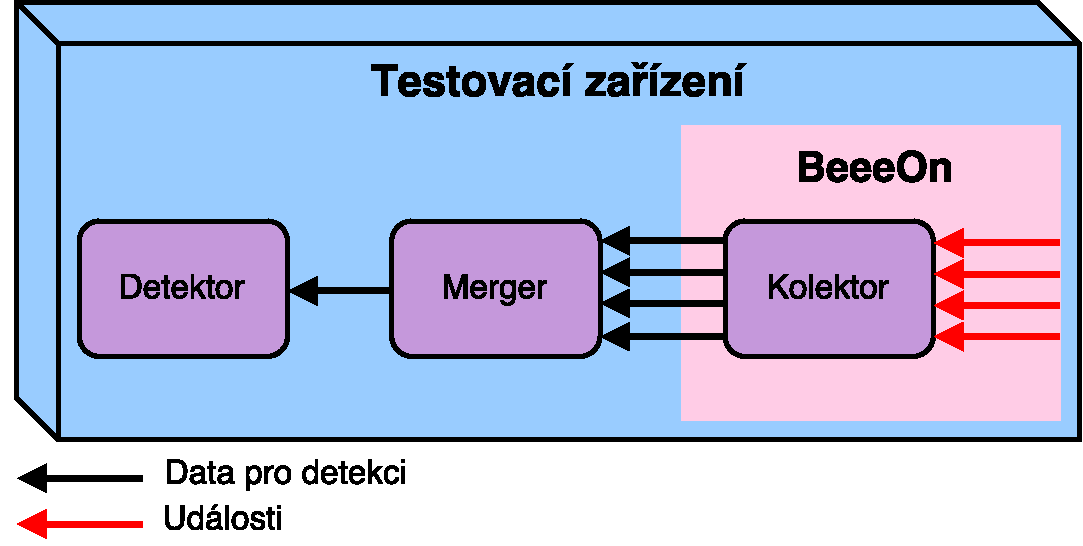
\includegraphics[scale=0.5]{pictures/deploy-option1}
   \caption{Lokální nasazení}
   \label{obr.option1}
   \end{center}
   \end{figure}
   
   Kolektor odesílá vždy dostupné události specifikovanými výstupními rozhraními dle konfigurace brány.
   Exporovaná data přijímá NEMEA modul \textit{Merger}, který je spojuje a předává detektoru.
   
  \item \textbf{Oddělený režim}
  
  Druhý způsob nasazení byl také otestován na lokálním zařízení, protože lze využít lokálních
  soketů, které nabízí NEMEA framework. Způsob zavedení je na obrázku \ref{obr.option2}.
 
  \begin{figure}[ht]
   \begin{center}
   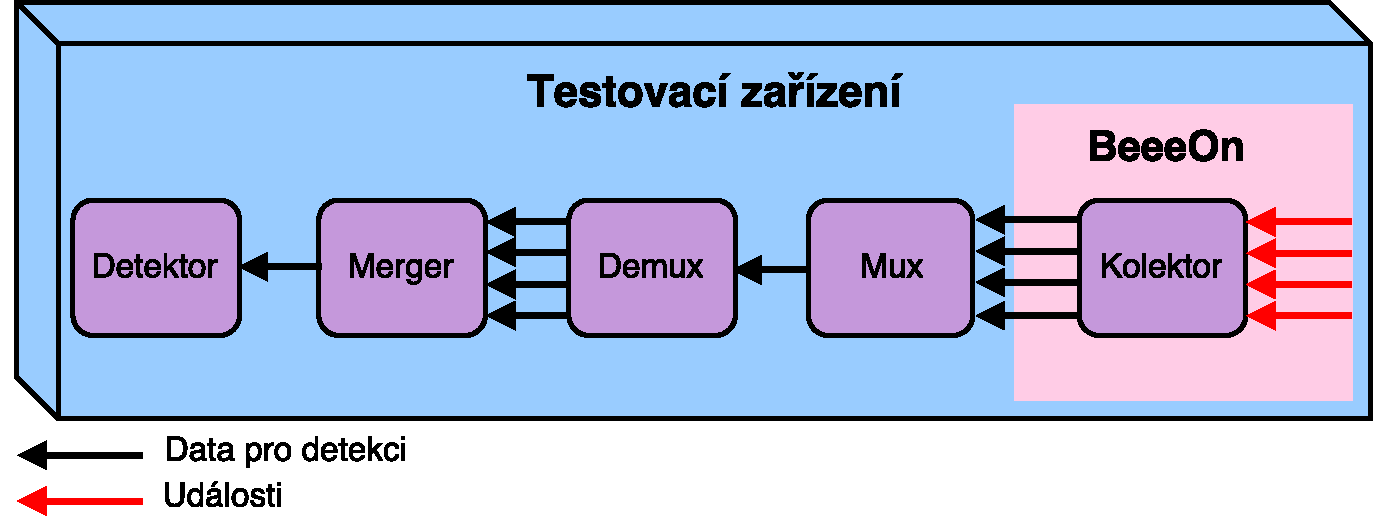
\includegraphics[scale=0.5]{pictures/deploy-option2}
   \caption{Oddělené nasazení}
   \label{obr.option2}
   \end{center}
   \end{figure}
   
   Složení komponent vychází z prvního případu, který byl rozšířen o moduly Mux a Demux, které 
   umí spojit a rozdělit přicházející komunikaci.
 \end{itemize}
 
Cílem testů bylo, aby detektor obdržel všechny odeslané zprávy z kolektoru. Ověření bylo provedeno
spuštěním detektoru s přepínačem \textit{-vv}, který zapne ladící výpisy druhé úrovně pro zobrazení 
přijatých UniRec polí. Výsledky obou případů byly úspěšné a všechna data byla přijata.

\section{Detekce scénářů útoků}
Velmi důležitou částí bylo otestování definovaných anomálií, které mohou reprezentovat skutečný
útok na sít. Tato sekce popisuje testy pro jednotlivé scénáře.

  \begin{enumerate}
    \item \textbf{Periodicita dat}
    
    Tento scénář nebylo nutné dělit na jednotlivé protokoly, protože popisuje obecné chování 
    připojených senzorů bez ohledu na technologii. Cílem bylo odhalit provoz, který porušuje
    očekávaný periodický průběr. V rámci detekce nebyly potřebné naučené profily sítě, 
    ale využívalo se parametrů ze skupiny \textit{general} umožňující periodické kontroly.
    
    První test byl určený na odhalení nepravidelného přijetí dat. Pro ověření byla použita událost
    \textit{onExport}, která poskytuje hodnoty získané ze senzorů, a v konfiguračním souboru byla 
    aktivována pravidelná kontrola dat každých 8 sekund.
    
    Výsledek testu byl úspěšný. Pokud nebyla obdžena žádná data déle než 8 sekund, tak byly
    odeslány informace o incidentu.
    
    Několik událostí poskytovaných branou BeeeOn jsou čistě periodické a po uplynutí definovaného
    času vždy odešlou dostupné statistiky. Druhý test byl zaměřen na odhalení případu, kdy se 
    přijímané datové položky nemění, což může reprezentovat odpojení nebo ztrátu čidla. Pro 
    otestování byla zvolena událost \textit{onHciStats}, které získává informace o provozu BLE sítě. 
    Dále byla v konfiguračním souboru nastavena pravidelná kontrola dat na 7 sekund a maximálně 
    5 po sobě přijatých hodnot mohlo být stejných. 
    
    Výsledek byl pozitivní, protože při přijetí více než pěti stejných po sobě jdoucích
    hodnot byla detekována anomálie.
    
    \item \textbf{Množství přenášených zpráv}
    
    V případě protokolu Z-Wave byly pro nasimulování anomálií použity dvě vzdáleně ovladatelné
    zásuvky. Obě mají k dispozici ovládací tlačítko pro vypnutí a zapnutí zásuvky. Tímto způsobem
    byly generovány nové zprávy. Cílem tohoto scénáře bylo odhalit neočekávaný nárůst dat, proto
    byla zvolena detekční metoda, která hlídá tyto změny. V rámci testu byly do profilu 
    vloženy všechny dostupné položky. Limitem pro ohlášení incidentu byl pětinásobný nárůst
    provozu. Délka časové řady byla nastavena na deset prvků a prvních jedenáct přijatých 
    zpráv bylo ignorováno, protože během nich bylo navazováno spojení.
    
    První detekce byla zaměřena na položku \textit{SOAFCount}, která určuje celkový počet 
    detekovaných zpráv.  
    Druhý scénář sledoval hodnotu \textit{receivedCount}, která reprezentuje počet přijatých zpráv od
    konkrétního čidla. 
    
    Pro BLE byla časová řada zkrácena na pět prvků, žádné zprávy nebyly ignorovány a limitem
    pro určení anomálie byl dvojnásobný nárůst dat.
    Test byl proveden pro položku \textit{rxBytes}, která určuje množtví obdržených zpráv.
    Data byly vyčítány skriptem, který v čase měnil četnost zaslaných požadavků o data.
    
    Výsledky testů byly úspěšné a každá změna provozu byla odhalena. Průběh všech testovaných
    případů byl velmi podobný a lišil se jen typ události a způsob generování dat. Chování 
    jednotlivých položek profilu velmi ovlivňovala délka časové řady, která určovala 
    paměťové okno. Nejcitlivější položkou na změnu byl rozptyl, který výrazně zvyšoval
    svou hodnotu při vložení vyššího čísla. K častým výchylkám docházelo i v případě průměru. 
    Méně frekventované změny nastávaly u mediánu, který nejvíce využíval délky časové řady. 
    Nejmenších odlišností dosahoval klouzavý průměr, protože ve své hodnotě obsahuje i data
    mimo aktuální časové okno.

    \item \textbf{Limity senzorových hodnot}
    
    Pro tento scénář byla použita data vygerovaná virtuálními senzory, které jsou dostupné
    v rámci brány BeeeOn. Do konfiguračního profilu byly vloženy všechny položky, pro které
    byly specifikovány parametry pro očekávané soft a hard limity. Cílem scénáře bylo odhalení
    změn v aktuálním profilu provozu, které porušují předepsané limity. 
    
    Výsledek detekce splnil očekávání a nepovolené změny byly úspěšně detekovány. Chování 
    jednotlivých položek profilu se shodovalo s předchozím scénářem.
    
    \item \textbf{Kvalita přenosového kanálu}
    
    Cílem tohoto případu užití bylo detekování změny kvality přenosového kanálu. Pro Z-Wave jsou 
    k tomuto účelu vhodné položky \textit{lastResponseRTT} a \textit{dropped}. Údaj
    \textit{lastResponseRTT} je součástí události \textit{onNodeStats} a 
    \textit{dropped} je obsažen v \textit{onDriverStats}. Z tohoto důvodu byl při generování dat použit
    NEMEA modul \textit{Merger}, který spojil dvě různě události do jedné. V konfiguračním souboru
    bylo nutné popsat obě hodnoty. V případě \textit{lastResponseRTT} byla jako anomálie označena
    hodnota průměru časového okna přesahující dvojnásobek vzorovného profilu a nebo byla nižší
    než polovina původního průměru. Pro položku \textit{dropped} bylo jako incident považováno
    libovolné zvětšení mediánu. Proto byla velikost časového okna rovna jedné a limit hard limitu byl
    nastaven na jedna. 
    
    Jelikož došlo ke spojení dvou různých událostí, kde \textit{onNodeStats}
    umožňuje získat informace pro jednotlivé senzory a \textit{onDriverStats} pro celou síť, 
    tak výsledkem byla událost poskytující informace pro každý koncový prvek. Z tohoto důvodu 
    musel být v konfiguraci uveden indentifikátor příslušných zařízení určených k analýze.
    
    Výstupy detekce se shodovaly s předpoklady, a proto byl výsledek testu úspěšný. V současné
    době se zatím nepodařilo připravit zkušební prostředí, ve které by bylo možné otestovat
    rušení kanálu, a tím ovlivnit hodnotu \textit{lastResponseRTT}. Pro účely otestování 
    detekce však byla postačující ruční úprava dat v souboru se zachyceným provozem. 
    
    V případě BLE by se využily položky \textit{rxErrors} nebo \textit{txErrors} a nastavení 
    detekce by bylo shodné s \textit{lastResponseRTT}. Vzhledem k tomu, že by došlo jen 
    ke změně názvu klíče v konfiguračním souboru, tento test nebyl proveden.
    
    \item \textbf{Konektivita}
    
    Pro ověření posledního scénáře lze využít poznatků z předchozích testů. Ztráta konektivity
    může být způsobena neobržením očekávané události a to lze detekovat pomocí periodicity dat.
    Druhým způsobem je výrazné zhoršení statistik přenosového kanálu, které byly zpracovány
    v předchozím případu užití.
  \end{enumerate}
  
  Ověření definovaných scénářů umožnilo otestování správné funkcionality vytvořeného detekčíního
  systému a zároveň byla sestavena množina informací, kterou je nutné sledovat k získání 
  přehledu o stavu sítě.
  
  Vygenerovaný provoz, na kterém byly jednotlivé případy užití otestovány je uložen i s nalezenými
  anomáliemi a konfiguračním souborem na přiloženém CD. V případě testu periodicity dat nebylo možné záznam 
  komunikace uložit, protože použitá detekce využívá aktuální čas. Z tohoto důvodu 
  byl do souboru místo záznamu uložen popis, jak takový provoz vygenerovat.

\section{Test exportu dat}
Identifikované scénáře útoků otestovaly většinu funkcí detekčního systému. Vytvořený nástroj
ovšem posktuje i možnost pravidelného exportu definovaných položek aktuálního profilu, a tím 
vytváří informace pro další pokročilejší detekce. 

Sada tesů ověřila, že vypočítané části profilu lze spolehlivě exportovat. Výsledek byl tedy
pozitivní.

\section{Měření položek profilu}